\documentclass[a4paper]{article}
\usepackage[utf8]{inputenc}
\usepackage[spanish, es-tabla, es-noshorthands]{babel}
\usepackage[table,xcdraw]{xcolor}
\usepackage[a4paper, footnotesep = 1cm, width=20cm, top=2.5cm, height=25cm, textwidth=18cm, textheight=25cm]{geometry}
%\geometry{showframe}

\usepackage{tikz}
\usepackage{amsmath}
\usepackage{amsfonts}
\usepackage{amssymb}
\usepackage{float}
\usepackage{graphicx}
\usepackage{caption}
\usepackage{subcaption}
\usepackage{multicol}
\usepackage{multirow}
\setlength{\doublerulesep}{\arrayrulewidth}
\usepackage{booktabs}

\usepackage{hyperref}
\hypersetup{
    colorlinks=true,
    linkcolor=blue,
    filecolor=magenta,      
    urlcolor=blue,
    citecolor=blue,    
}

\newcommand{\quotes}[1]{``#1''}
\usepackage{array}
\newcolumntype{C}[1]{>{\centering\let\newline\\\arraybackslash\hspace{0pt}}m{#1}}
\usepackage[american]{circuitikz}
\usetikzlibrary{calc}
\usepackage{fancyhdr}
\usepackage{units} 

\graphicspath{{../Ejercicio-1/}{../Ejercicio-2/}}

\pagestyle{fancy}
\fancyhf{}
\lhead{22.67 - Señales Aleatorias}
\rhead{Lambertucci, Londero B., Moriconi, Musich, Tolaba}
\rfoot{Página \thepage}

\begin{document}

%%%%%%%%%%%%%%%%%%%%%%%%%
%		Caratula		%
%%%%%%%%%%%%%%%%%%%%%%%%%

\begin{titlepage}
\newcommand{\HRule}{\rule{\linewidth}{0.5mm}}
\center
\mbox{\textsc{\LARGE \bfseries {Instituto Tecnológico de Buenos Aires}}}\\[1.5cm]
\textsc{\Large 22.67 Señales Aleatorias}\\[0.5cm]


\HRule \\[0.6cm]
{ \Huge \bfseries Trabajo práctico N$^{\circ}$3}\\[0.4cm] 
\HRule \\[1.5cm]


{\large

\emph{Grupo 1:}\\
\vspace{3pt}

\begin{tabular}{lr} 	
\textsc{Lambertucci}, Guido Enrique  & 58009 \\
\textsc{Londero Bonaparte}, Tomás Guillermo  & 58150 \\
\textsc{Musich}, Francisco  & 58124\\
\end{tabular}

\vspace{20pt}

\emph{Profesor}\\
\textsc{Hirchoren}, Gustavo Abraham \\
\vspace{3pt}
%\textsc{} \\	

\vspace{100pt}

\begin{tabular}{ll}

Presentado: & 07/02/22\\

\end{tabular}

}

\vfill

\end{titlepage}


%%%%%%%%%%%%%%%%%%%%%
%		Indice		%
%%%%%%%%%%%%%%%%%%%%%

\tableofcontents
\newpage

%%%%%%%%%%%%%%%%%%%%%
%		Informe		%
%%%%%%%%%%%%%%%%%%%%%

\section{Ejercicio 1}
	\label{Ejercicio-1}
	\documentclass[a4paper]{article}
\usepackage[utf8]{inputenc}
\usepackage[spanish, es-tabla, es-noshorthands]{babel}
\usepackage[table,xcdraw]{xcolor}
\usepackage[a4paper, footnotesep = 1cm, width=20cm, top=2.5cm, height=25cm, textwidth=18cm, textheight=25cm]{geometry}
%\geometry{showframe}

\usepackage{tikz}
\usepackage{amsmath}
\usepackage{amsfonts}
\usepackage{amssymb}
\usepackage{float}
\usepackage{graphicx}
\usepackage{caption}
\usepackage{subcaption}
\usepackage{multicol}
\usepackage{multirow}
\setlength{\doublerulesep}{\arrayrulewidth}
\usepackage{booktabs}

\usepackage{hyperref}
\hypersetup{
    colorlinks=true,
    linkcolor=blue,
    filecolor=magenta,      
    urlcolor=blue,
    citecolor=blue,    
}

\newcommand{\quotes}[1]{``#1''}
\usepackage{array}
\newcolumntype{C}[1]{>{\centering\let\newline\\\arraybackslash\hspace{0pt}}m{#1}}
\usepackage[american]{circuitikz}
\usetikzlibrary{calc}
\usepackage{fancyhdr}
\usepackage{units} 

\graphicspath{{../Ejercicio-1/}{../Ejercicio-2/}}

\pagestyle{fancy}
\fancyhf{}
\lhead{22.67 - Señales Aleatorias}
\rhead{Lambertucci, Londero B., Moriconi, Musich, Tolaba}
\rfoot{Página \thepage}
\begin{document}
\subsection{Introducción}

El siguiente ejercicio parte de un análisis sobre el proceso aleatorio presente en la página 138 del libro selecto por la cátedra. Se realizarán simulaciones de dicho proceso y se calcularán experimentalmente la media, la varianza, la autocorrelación y el coeficiente de autocorrelación para ciertos valores de t dados y se realizará una comparación con los valores teóricos.

\subsection{Valores teóricos}

El experimento que determina el proceso es la tirada de un dado no cargado y el ensamble del mismo se detalla a continuación:
\begin{equation} 
	\begin{split}
		 &y_{1(t)} = 6 \\
		 &y_{2(t)} = 3sin(t) \\
		 &y_{3(t)} = -3sin(t) \\
		 &y_{4(t)} = 3cos(t) \\
		 &y_{5(t)} = -3cos(t) \\
		 &y_{6(t)} = -6
	\end{split}
\end{equation}

El proceso es $Y_{(t)} = y_{i(t)}$ donde i indica el número obtenido en la tirada del dado.\\

El valor esperado teórico del proceso se obtiene de la siguiente forma:

\begin{equation*}
\begin{gathered}
	E\left[Y_{(t)}\right] = \sum_{i=1}^{6}\left( P(Y_{(t)} = y_{i(t)}) \times y_{i(t)}\right) 
\end{gathered}
\end{equation*}

Reemplazando las funciones muestra dadas y que la probabilidad $P(Y_{(t)} = y_{i(t)})= \frac{1}{6}$ $ \forall i $ obtenemos que:	

\begin{equation*}
\begin{gathered}
	E\left[Y_{(t)}\right] = 0$ $\forall t 
\end{gathered}
\end{equation*}

La varianza se obtiene como:

\begin{equation*}
\begin{gathered}
	Var^{2}_{(t)} = E\left[Y_{(t)}^{2}\right]- \left(E\left[Y_{(t)}\right]\right)^{2}  = \sum_{i=1}^{6}\left( P(Y_{(t)} = y_{i(t)}) \times y_{i(t)}^{2}\right) - 0^2 = 15 $   $ \forall t 
\end{gathered}
\end{equation*}

Donde ya se obtuvo que $E\left[Y_{(t)}\right] = 0$ y 

\begin{equation*}
\begin{gathered}
	E\left[Y_{(t)}^{2}\right] = \sum_{i=1}^{6}\left( P(Y_{(t)} = y_{i(t)}) \times y_{i(t)}^{2}\right) 
\end{gathered}
\end{equation*}

Este proceso tiene media y "varianza" constantes para todo instante t.

La autocorrelación para dos instantes t1 y t2 se encuetra calculada en el libro y nos queda como:
\begin{equation*}
\begin{gathered}
	R_{xx(t_1,t_2)} = \frac{1}{6}\left(72+ 18 \cos(t_2 - t_1)\right)
\end{gathered}
\end{equation*}

El proceso tiene media constante y autocorrelación dependiente de $(t_2 - t_1)$, entonces es WSS. Por lo tanto:
\begin{equation*}
\begin{gathered}
	R_{xx(t,t)} = R_{xx(0,0)} = \frac{1}{6}\left(72+ 18 \cos(0)\right) = 15
\end{gathered}
\end{equation*}

El coeficiente de autocorrelación se obtiene con la definición del mismo:
\begin{equation*}
\begin{gathered}
	r_{xx(t_1,t_2)} = \frac{R_{xx(t_1,t_2)}-\mu_{X_{(t_1)}}^{*} \mu_{X_{(t_2)}}}{\left(R_{xx(t_1,t_1)}.R_{xx(t_2,t_2)}\right)^{1/2}} 
\end{gathered}
\end{equation*}

Como el proceso es WSS y su media es cero cualquiera sea t:

\begin{equation*}
\begin{gathered}
	r_{xx(t_1,t_2)} = \frac{R_{xx(t_1,t_2)}-0}{(R_{xx(0,0)}^2)^{1/2}} = \frac{\frac{1}{6}\left(72+ 18 \cos(t_2 - t_1)\right)}{15}
\end{gathered}
\end{equation*}\\


Para los instantes de t requeridos, obtenemos los siguientes resultados:
\begin{enumerate}
	\item[•]E$\left[ Y_{(\frac{\pi}{2})}\right]$= 0 
	\item[•]Var$\left[Y_{(\frac{\pi}{2})}\right]$= 15
	\item[•]$R_{xx(\frac{\pi}{4},\frac{\pi}{2})}$= $\frac{1}{6} (72 + 18 \cos(\frac{\pi}{4}))$ = 14.12132
	\item[•]$r_{xx(2\pi,\pi)} = \frac{R_{xx(\pi,2\pi)}}{15} = \frac{ (12 + 3 \cos(\pi))}{15}$ = 0.6 \\
\end{enumerate}

Observando el ensamble dado se puede comprobar fácilmente que el proceso no es ergódico en la media puesto que con la función muestra $y_{1(t)} = 6$:

\begin{equation*}
\begin{split}
	\lim_{T\to\infty} < Y_{(t)} >_T = & \lim_{T\to\infty} \frac{1}{T} \int_{-T/2}^{T/2} Y(t) dt  \neq \mu 
\end{split}
\end{equation*}

De la misma forma, se puede concluir que no es ergódico en la autocorrelación con la misma función muestra:

\begin{equation*}
\begin{split}
	\lim_{T\to\infty} < R_{YY}(\tau) >_T = & \lim_{T\to\infty} \frac{1}{T} \int_{-T/2}^{T/2} Y(t) Y(t + \tau) dt \neq R{YY}(\tau) \ 	\forall \tau
\end{split}	
\end{equation*}
%\underbrace{\frac{1}{6}}{y_1(t)}
Dado que para una de las funciones no se cumple que tienda a la autocorrelación, no es ergódico en en dicha variable.\\


\subsection{Análisis Experimental}

Para el análisis sobre los valores pedidos es necesario generar múltiples muestras sobre el proceso, en los instantes de tiempo requeridos. En primer lugar, se obtiene un número entero al azar entre 1 y 6, simulando la tirada de un dado, el cual determina qué función miembro del ensamble resulta.
A partir de la determinacion de la función correspondiente se evalua en los valores de instantes t pedidos, obteniendose:

\begin{enumerate}
   \item[•] $Y(\pi/2)$
   \item[•] $Y(\pi/4)$
   \item[•] $Y(\pi)$
   \item[•] $Y(2\pi)$
\end{enumerate}

Estos valores obtenidos se guardan como un vector. Luego, se repite el procedimiento N = 1000 veces 
y se obtiene un arreglo de vectores conteniendo muestras del proceso.
El codigo de Matlab empleado para la simulaci[on de este proceso se detalla a continuaci[on 
\\

\begin{figure}[H]
\centering
	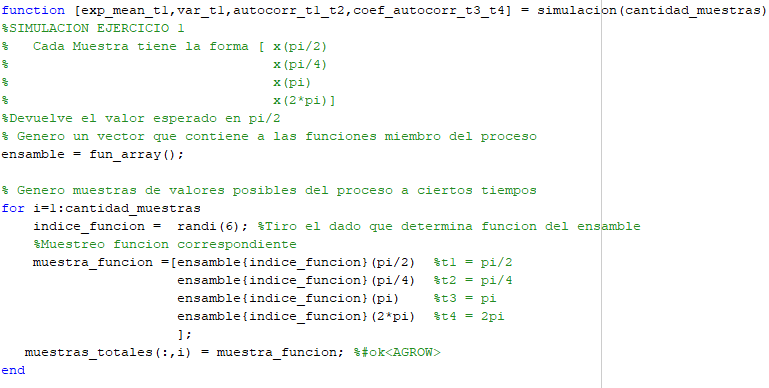
\includegraphics[width=0.8\textwidth, trim = {0 0 0 0},clip]{./ImagenesEjercicio1/main1.png}
	\caption{Código Matlab de la simulación del proceso.}
	\label{fig:main1}
\end{figure}

Donde la funcion fun-array() designa el ensamble solicitado, el c[odigo en Matlab:

\begin{figure}[H]
\centering
	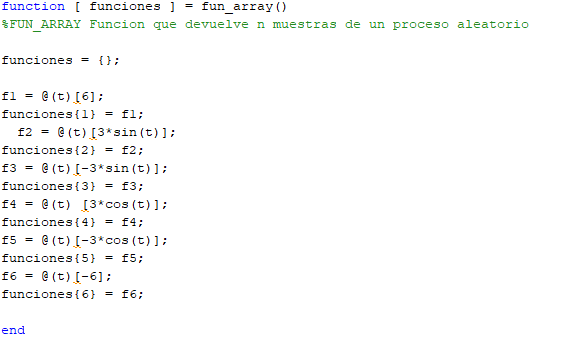
\includegraphics[width=0.6\textwidth, trim = {0 0 0 0},clip]{./ImagenesEjercicio1/fun_array.png}
	\caption{La función que contiene el ensamble del proceso.}
	\label{fig:fun_array}
\end{figure}

A continuación, por ejemplo se muestran los resultados para $Y(\pi/2)$ para N = 100 experimentos realizados.

\begin{figure}[H]
\centering
	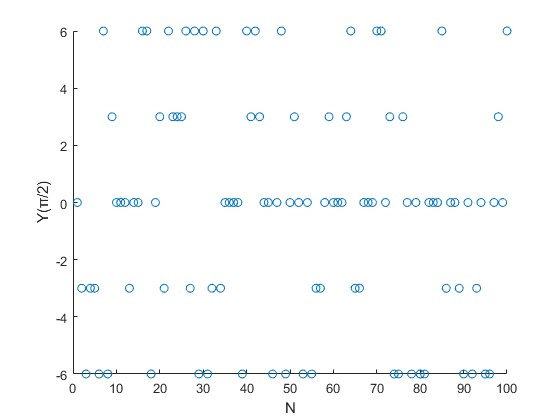
\includegraphics[width=0.4\textwidth, trim = {0 0 0 0},clip]{./ImagenesEjercicio1/ypi_2.png}
	\caption{Valores del proceso $Y_(t)$ en $t = \frac{\pi}{2} $.}
	\label{fig:ypi_2}
\end{figure}

También para $Y(\pi/4)$.

\begin{figure}[H]
\centering
	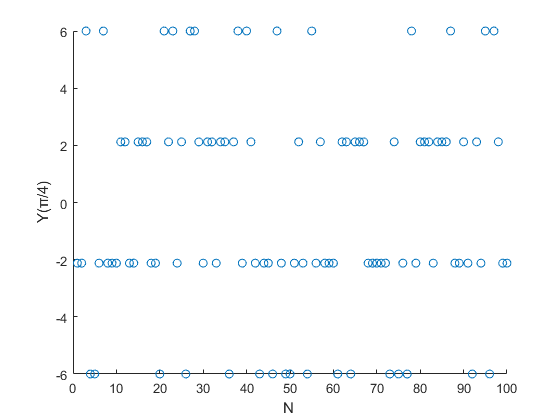
\includegraphics[width=0.4\textwidth, trim = {0 0 0 0},clip]{./ImagenesEjercicio1/ypi_4.png}
	\caption{Valores del proceso $Y_(t)$ en $t = \frac{\pi}{4} $.}
	\label{fig:ypi_4}
\end{figure}

Luego, se calculan promediando los valores pedidos con el código:

\begin{figure}[H]
\centering
	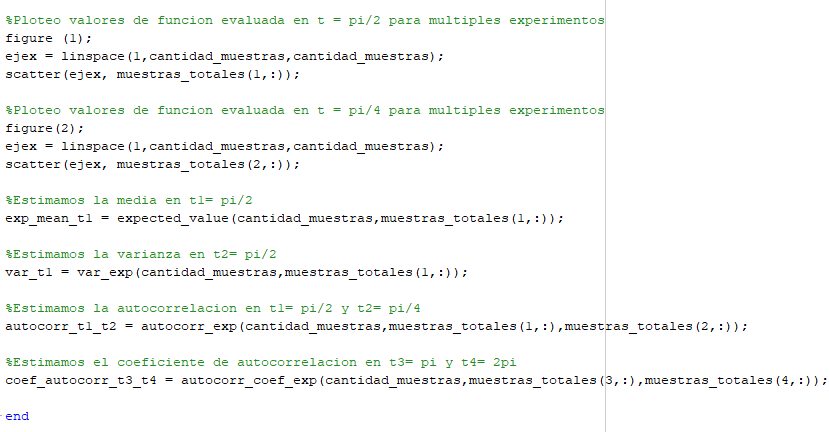
\includegraphics[width=0.8\textwidth, trim = {0 0 0 0},clip]{./ImagenesEjercicio1/main2.png}
	\caption{Código de Matlab de la simulación del proceso.}
	\label{fig:main2}
\end{figure}

Detallando cada función:
\begin{enumerate}
\item[•] La funcio[n estimadora de la media en $t = \frac{\pi}{2}$, E$\left[ Y_{(\frac{\pi}{2})}\right]$
\begin{figure}[H]
\centering
	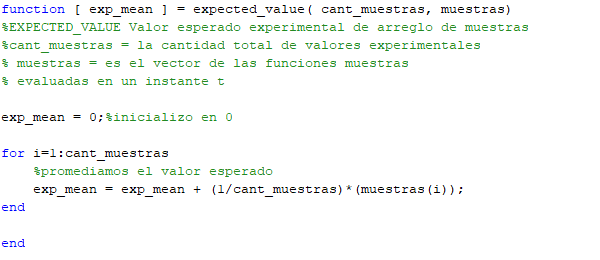
\includegraphics[width=0.6\textwidth, trim = {0 0 0 0},clip]{./ImagenesEjercicio1/expval.png}
	\caption{La función que calcula la media experimental del proceso.}
	\label{fig:expval}
\end{figure}

\item[•] La función estimadora de la varianza en $t = \frac{\pi}{2}$, Var$\left[Y_{(\frac{\pi}{2})}\right]$
\begin{figure}[H]
\centering
	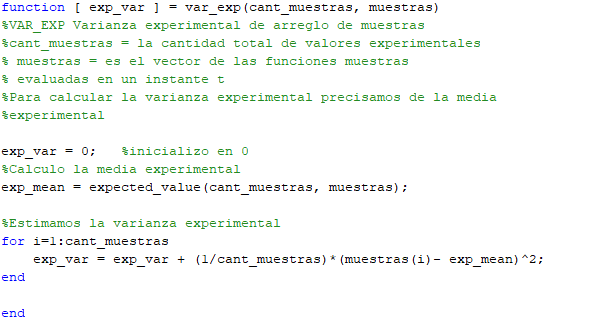
\includegraphics[width=0.6\textwidth, trim = {0 0 0 0},clip]{./ImagenesEjercicio1/expvar.png}
	\caption{La función que calcula la varianza experimental.}
	\label{fig:expvar}
\end{figure}

\item[•] La función estimadora de la autocorrelación en $t_1 = \frac{\pi}{4}$ y $t_2 = \frac{\pi}{2}$, $R_{xx(\frac{\pi}{4},\frac{\pi}{2})}$
\begin{figure}[H]
\centering
	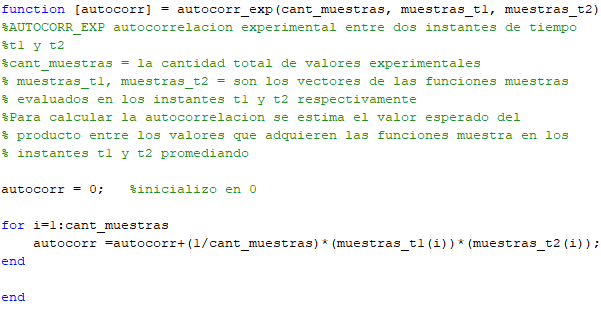
\includegraphics[width=0.6\textwidth, trim = {0 0 0 0},clip]{./ImagenesEjercicio1/autocorr.png}
	\caption{La función estimadora de la autocorrelación.}
	\label{fig:autocorr}
\end{figure}

\item[•] La función estimadora del coeficiente de autocorrelación en $t_3 = \frac{2\pi}{4}$ y $t_4 = \pi$, $r_{xx(2\pi,\pi)}$
\begin{figure}[H]
\centering
	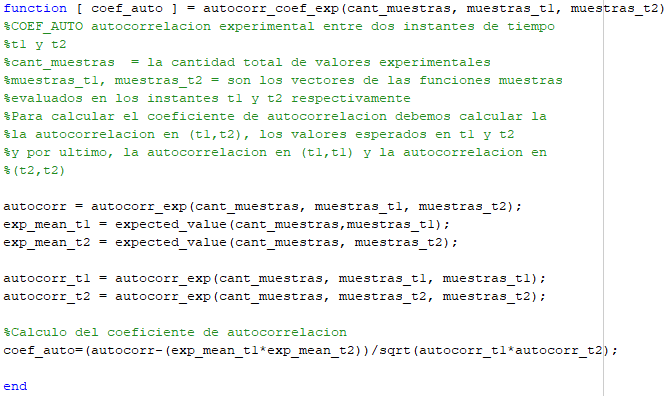
\includegraphics[width=0.6\textwidth, trim = {0 0 0 0},clip]{./ImagenesEjercicio1/coefauto.png}
	\caption{La función estimadora del coeficiente de autocorrelación.}
	\label{fig:coefauto}
\end{figure}
\end{enumerate}

Corriendo la simulación para N = 1000, se arrojaron los siguientes resultados:
\begin{figure}[H]
\centering
	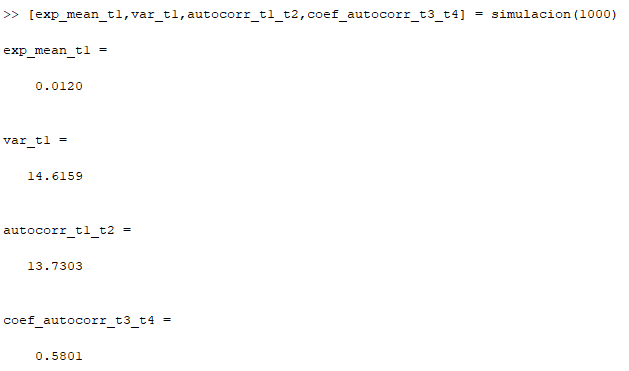
\includegraphics[width=0.6\textwidth, trim = {0 0 0 0},clip]{./ImagenesEjercicio1/result.png}
	\caption{Resultados de la simulación con N = 1000 muestras}
	\label{fig:result}
\end{figure}

Observando la figura (\ref{fig:result}) obtenemos que:
\begin{enumerate}
	\item[•]E$\left[ Y_{(\frac{\pi}{2})}\right]$= 0.0120 
	\item[•]Var$\left[Y_{(\frac{\pi}{2})}\right]$= 14.6159
	\item[•]$R_{xx(\frac{\pi}{4},\frac{\pi}{2})}$= 13.7303
	\item[•]$r_{xx(2\pi,\pi)}$= 0.5801
\end{enumerate}

Adicionalemente, analizamos para la media en $t_1 = \frac{\pi}{2}$ que E$\left[ Y_{(\frac{\pi}{2})}\right]\rightarrow 0$ a medida que se realizan simulaciones con N$\rightarrow \infty$
\begin{figure}[H]
\centering
	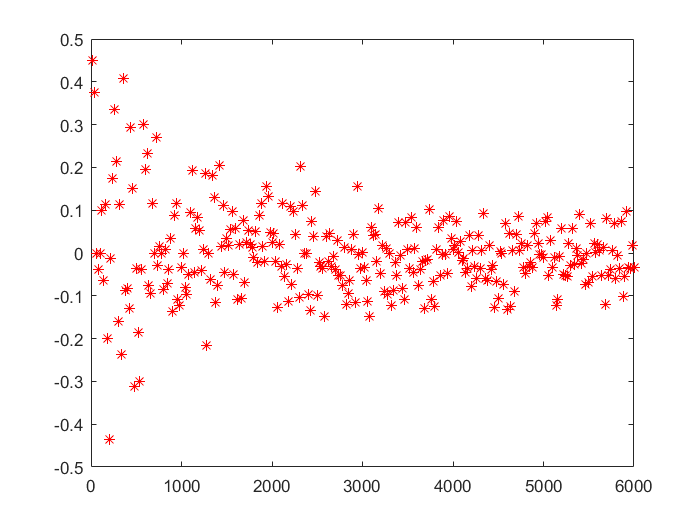
\includegraphics[width=0.6\textwidth, trim = {0 0 0 0},clip]{./ImagenesEjercicio1/media.png}
	\caption{El valor esperado del proceso en $t_1 = \frac{\pi}{2}$ cuando la cantidad de muetras aumenta.}
	\label{fig:media}
\end{figure}

\subsection{Conclusiones sobre los resultados}

En primer lugar, en las figuras (\ref{fig:ypi_2}) y (\ref{fig:ypi_4}) se puede "estimar" visualmente que la media para el proceso es cero como primer aproximación a los valores teóricos.

Luego, se puede concluir que para los valores experimentales, la media en $t_1 = \frac{\pi}{2}$ es cercana a cero y a medida que aumentamos la cantidad de valores muestreados la diferencia entre el valor experimental y el valor teórico es cada vez más pequeña. De igual manera, para la varianza en $t_1 = \frac{\pi}{2}$, no se observan diferencias significativas.
También, la autocorrelación en $t_1 = \frac{\pi}{2}$ y $t_2 = \frac{\pi}{4}$ y la autocorrelación en $t_3 = \pi$ y $t_4 = 2\pi$ denotan el mismo comportamiento hacia el valor teórico. 

A medida que se toman mayor cantidad de muestras $(N \rightarrow \infty )$ los valores que se estimaron convergieron a los valores teoricos, lo cual era de esperarse puesto que el proceso tiene un ensamble simétrico y equiprobable. 

Los valores estimados con los muestreos del proceso no pueden estimarse mediante promedios temporales eligiendo alguna de las funciones muestras experimentales porque el proceso no es ergódico en la media ni tampoco en la autocorrelación. Esto puede observarse facilmente cuando el experimento aleatorio que determina el proceso cae en los valores de $y_{1(t)} = 6$ o $y_{6(t)} = -6$ 




\end{document}

\newpage
\section{Ejercicio 2}
	\label{Ejercicio-2}
	%\documentclass[a4paper]{article}
\usepackage[utf8]{inputenc}
\usepackage[spanish, es-tabla, es-noshorthands]{babel}
\usepackage[table,xcdraw]{xcolor}
\usepackage[a4paper, footnotesep = 1cm, width=20cm, top=2.5cm, height=25cm, textwidth=18cm, textheight=25cm]{geometry}
%\geometry{showframe}

\usepackage{tikz}
\usepackage{amsmath}
\usepackage{amsfonts}
\usepackage{amssymb}
\usepackage{float}
\usepackage{graphicx}
\usepackage{caption}
\usepackage{subcaption}
\usepackage{multicol}
\usepackage{multirow}
\setlength{\doublerulesep}{\arrayrulewidth}
\usepackage{booktabs}

\usepackage{hyperref}
\hypersetup{
    colorlinks=true,
    linkcolor=blue,
    filecolor=magenta,      
    urlcolor=blue,
    citecolor=blue,    
}

\newcommand{\quotes}[1]{``#1''}
\usepackage{array}
\newcolumntype{C}[1]{>{\centering\let\newline\\\arraybackslash\hspace{0pt}}m{#1}}
\usepackage[american]{circuitikz}
\usetikzlibrary{calc}
\usepackage{fancyhdr}
\usepackage{units} 

\graphicspath{{../Ejercicio-1/}{../Ejercicio-2/}}

\pagestyle{fancy}
\fancyhf{}
\lhead{22.67 - Señales Aleatorias}
\rhead{Lambertucci, Londero B., Moriconi, Musich, Tolaba}
\rfoot{Página \thepage}
%
%\begin{document}

\subsection{Introducción}

Se analiza una secuencia $X(n)$, estimando y calculando parámetros de interés, como lo son la autocorrelación, los coeficientes de correlación parcial y la densidad espectral de potencia.

\subsection{Autocorrelación} 

Se estiman la autocorrelación mediante el uso de los primeros $128$ elementos de la secuencia brindada. Para ello, se vale los estimadores polarizados ($R_{p}$) y no polarizados ($R_{np}$) de dicho parámetro. Estas funciones son las empleadas para estimar otras funciones mediante información digitalizada.
\begin{equation}
\begin{gathered}
	R_{p}(k) = \frac{1}{N} \sum_{i=0}^{N-k-1} X(i)X(i+k)	\\
	R_{np}(k) = \frac{1}{N-k} \sum_{i=0}^{N-k-1} X(i)X(i+k)
\end{gathered}
\end{equation}
En ellas se observan los parámetros $N$, es decir, el largo de $X(n)$, y $k$, variable que puede tomar los valores $0, 1, ... \ , 127$. Mediante el uso de estos estimadores, se normaliza para poder obtener los coeficientes de autocorrelación $r_{XXp}$ y $r_{XXnp}$. 

\begin{figure}[H]
\centering
	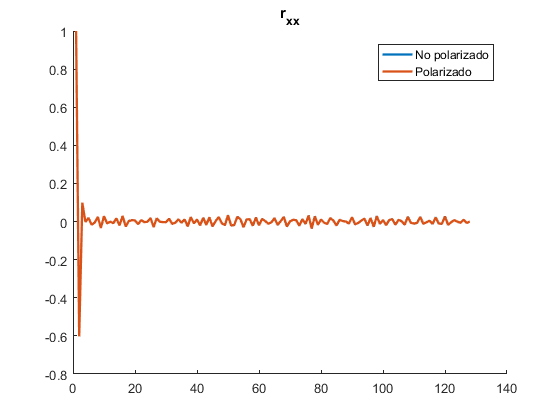
\includegraphics[width=0.8\textwidth, trim = {0 0 0 0.7cm},clip]{./ImagenesEjercicio2/rxx.png}
	\caption{Grafica de los coeficientes de autocorrelación total estimados.}
	\label{fig:rxx}
\end{figure}

Se puede observar en la Figura (\ref{fig:rxx}) como ambas curvas se encuentran solapadas, haciendo que sea prácticamente imposible distinguirlas.
Esto se debe a que existe una relación entre cada estimador, siendo esta
\begin{equation*}
\begin{gathered}
	R_{p}(k) = \frac{N - k}{N} R_{np}(k)
\end{gathered}
\end{equation*}

Ya que, para el caso del vector analizado, se da la condición de que $N = 4096$ y además $N >> k_{max} = 127$, siendo entonces
\begin{equation*}
\begin{gathered}
	R_{p}(k) \approx R_{np}(k)
\end{gathered}
\end{equation*}

\subsection{Coeficientes de correlación parcial}

Con los datos ya extraídos y mediante la resolución de la ecuación de Yule-Walker, fue posible obtener los coeficientes deseados. Esto se realizó con los coeficientes totales obtenidos a través de las estimaciones polarizada y no polarizada.
\begin{figure}[H]
\centering
	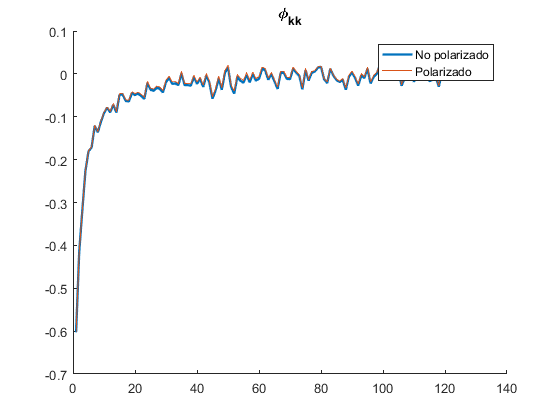
\includegraphics[width=0.7\textwidth, trim = {0 0 0 0.7cm},clip]{./ImagenesEjercicio2/phikk.png}
	\caption{Grafica de los coeficientes de autocorrelación parcial obtenidos.}
	\label{fig:phikk}
\end{figure}

En la Figura (\ref{fig:phikk}) se obtuvo nuevamente una diferencia entre ambas curvas, la cual no es significativa.

\subsection{Modelo del proceso}
\label{subsec:modelo}

Se procede a determinar que tipo de modelo utilizar para el proceso analizado. Observando la Figura (\ref{fig:rxx}), se denota que $r_{XX}(1)$ y $r_{XX}(2)$ son valores distintos de 0 ($-0,603$ y $0,099$ para ambas aproximaciones), mientras que los valores siguientes, si bien no son exactamente 0, son todos menores en modulo a $0,03$, lo que permite aproximarlos a 0. Además, observando la Figura (\ref{fig:phikk}), se puede afirmar que los $\phi_{kk}$ presentan un comportamiento exponencial. Es por ello que se determina que el proceso es un \textbf{MA(2)} (\textbf{ARMA(0,2)}).

Para el calculo de los $\theta$, se utilizaron las ecuaciones
\begin{equation}
	r_{XX}(1) = \frac{R_{XX}(1)}{\sigma_X^2} = \frac{\theta_{2,1} + \theta_{2,1} \theta_{2,2}}{1 +\theta_{2,1}^2 + \theta_{2,2}^2}
\end{equation}
\begin{equation}
	r_{XX}(2) = \frac{\theta_{2,2}}{1 +\theta_{2,1}^2 + \theta_{2,2}^2}
\end{equation}

Resolviendo dicho sistema, se obtienen los siguientes valores:
\begin{equation}
\begin{gathered}
	\theta_{2,1} = -1,280	\\
	\theta_{2,2} = 0,268	
\end{gathered}
\end{equation}

Con lo ya dicho, se procede a estimar los parámetros del proceso y compararlos con los ya obtenidos.

\begin{figure}[H]
\centering
	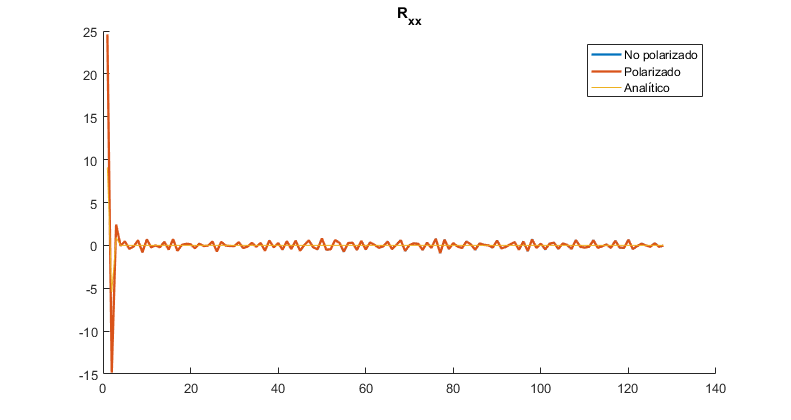
\includegraphics[width=0.8\textwidth, trim = {0 0 0 0.7cm},clip]{./ImagenesEjercicio2/Rxxcalc.png}
	\caption{Comparación de los coeficientes de autocorrelación.}
	\label{fig:Rxxcalc}
\end{figure}
\begin{figure}[H]
\centering
	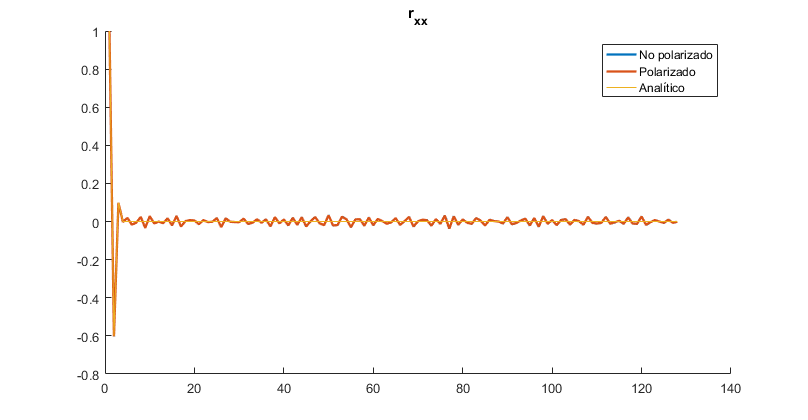
\includegraphics[width=0.8\textwidth, trim = {0 0 0 0.7cm},clip]{./ImagenesEjercicio2/rrxxcalc.png}
	\caption{Comparación de los coeficientes de autocorrelación normalizados.}
	\label{fig:rrxxcalc2}
\end{figure}

\subsection{Densidad espectral de potencia}

A continuación, se estima la la densidad espectral de potencia del vector $X(n)$. Para ello, se emplean dos técnicas distintas. La primera consiste en el uso de la transformada de Fourier de la estimación realizada de las funciones de autocorrelación.
\begin{figure}[H]
\centering
	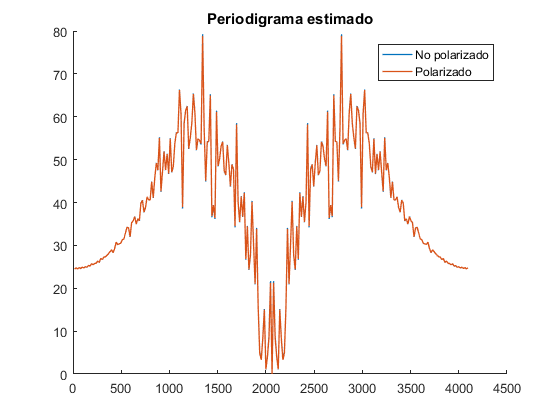
\includegraphics[width=0.8\textwidth, trim = {0 0 0 0.735cm},clip]{./ImagenesEjercicio2/period-est.png}
	\caption{Periodigramas obtenidos a partir de las estimaciones de $R_{XX}$.}
	\label{fig:period-est}
\end{figure}

%A continuación se comparan los estimaciones obtenidas previamente con la curva obtenida a partir de lo calculado en la Subsección (\ref{subsec:modelo}).
%\begin{figure}[H]
%\centering
%	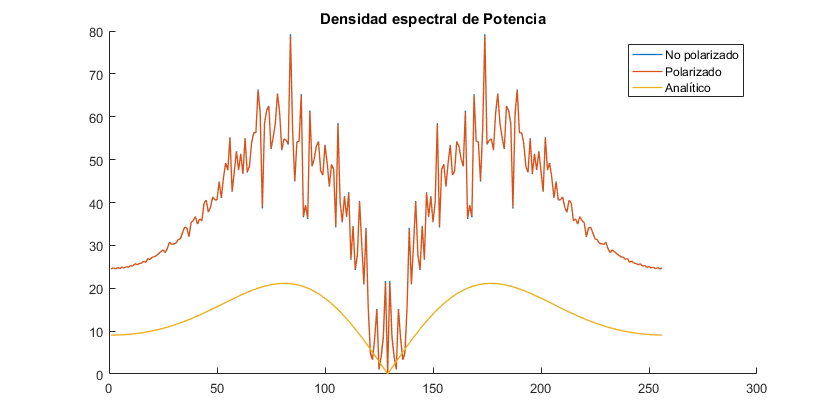
\includegraphics[width=0.7\textwidth, trim = {0 0 0 0.725cm},clip]{./ImagenesEjercicio2/densidadPot.png}
%	\caption{Comparación de periodigramas.}
%	\label{fig:densidadPot}
%\end{figure}

Como era de esperarse, la diferencia entre el gráfico obtenido a través de la estimación polarizada no difiere tanto de la no polarizada.

La segunda técnica consta de la promediación de periodigramas. Para esto se partió el vector original en 16 grupos de 256 elementos, en cada grupo se calculó los primeros 128 valores de la autocorrelacion con el estimador no polarizado, luego a cada vector se le calcula la densidad espectral de potencia y finalmente se las promedia.\footnote{Se utilizó la formula 9.24 del libro}
\begin{figure}[H]
\centering
	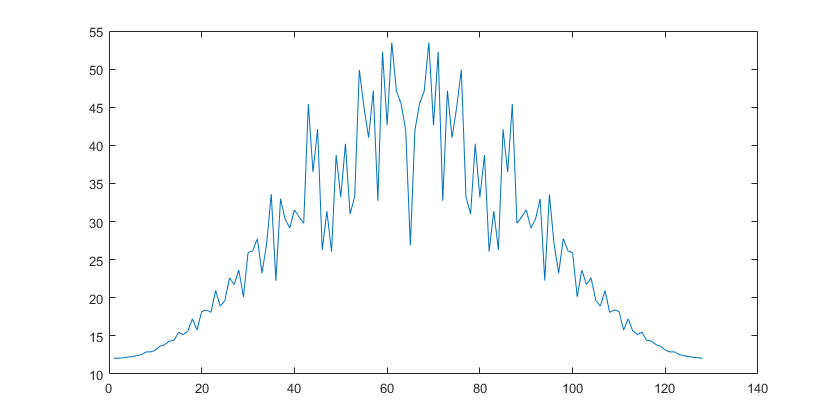
\includegraphics[width=0.8\textwidth, trim = {0 0 0 0.725cm},clip]{./ImagenesEjercicio2/period-calc.png}
	\caption{Estimación de la densidad espectral de potencia mediante el uso de promediación de periodigramas.}
	\label{fig:fft-calc}
\end{figure}



Finalmente, a modo comparativo, se ilustran las estimaciones obtenidas superpuestas:
\begin{figure}[H]
\centering
	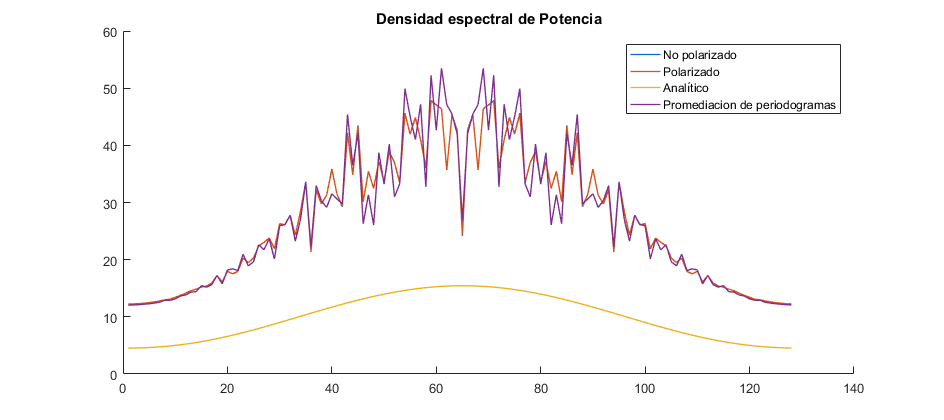
\includegraphics[width=0.8\textwidth, trim = {0 0 0 0.725cm},clip]{./ImagenesEjercicio2/fft2.png}
	\caption{Estimaciones de potencia.}
	\label{fig:fft2}
\end{figure}
Se puede apreciar que son muy similares tanto la promediación de periodogramas con la transformada de la estimación de la función de autocorrelación.
%\end{document}

%\subsection{Código implementado}
%
%\begin{itemize}
%\item Main.m:
%	\lstinputlisting[language=Matlab]{../Ejercicio-2/Matlab/Main.m}
%	
%\item Cpar.m:
%	\lstinputlisting[language=Matlab]{../Ejercicio-2/Matlab/cpar.m}
%	
%\item Rnp.m:
%	\lstinputlisting[language=Matlab]{../Ejercicio-2/Matlab/Rnp.m}
%	
%\item Rp.m:
%	\lstinputlisting[language=Matlab]{../Ejercicio-2/Matlab/Rp.m}

\end{itemize}

\end{document}